\section{Architecture logicielle}

	Plutôt qu'implémenter les nouvelles fonctionnalités directement dans ADTool, nous avons fait le choix de créer un nouveau logiciel nommé \glasir{} qui utilisera cet éditeur d'arbres. Deux raisons nous ont poussés à prendre cette décision. La première est de séparer l'analyse et l'édition des ADTrees, afin d'avoir des logiciels dédiés à leur tâche. De plus, cette solution nous permet d'utiliser des technologies différentes de celles d'ADTool, enrichissant ainsi notre formation. \glasir{} se chargera de la partie \textit{analyse}, et ADTool de la partie \textit{édition des arbres} sous forme de sous-fenêtre de \glasir{}. On peut voir sur la {\sc Figure} \ref{fig:architecture_Glasir} l'intégration d'ADTool dans l'architecture de \glasir. 
	% changer l'ordre ?
	% donner un nom au module du paramètre de ssynthése ?
	% oublier cette histoire de module ?

	\begin{figure}[h!]
		\centering
			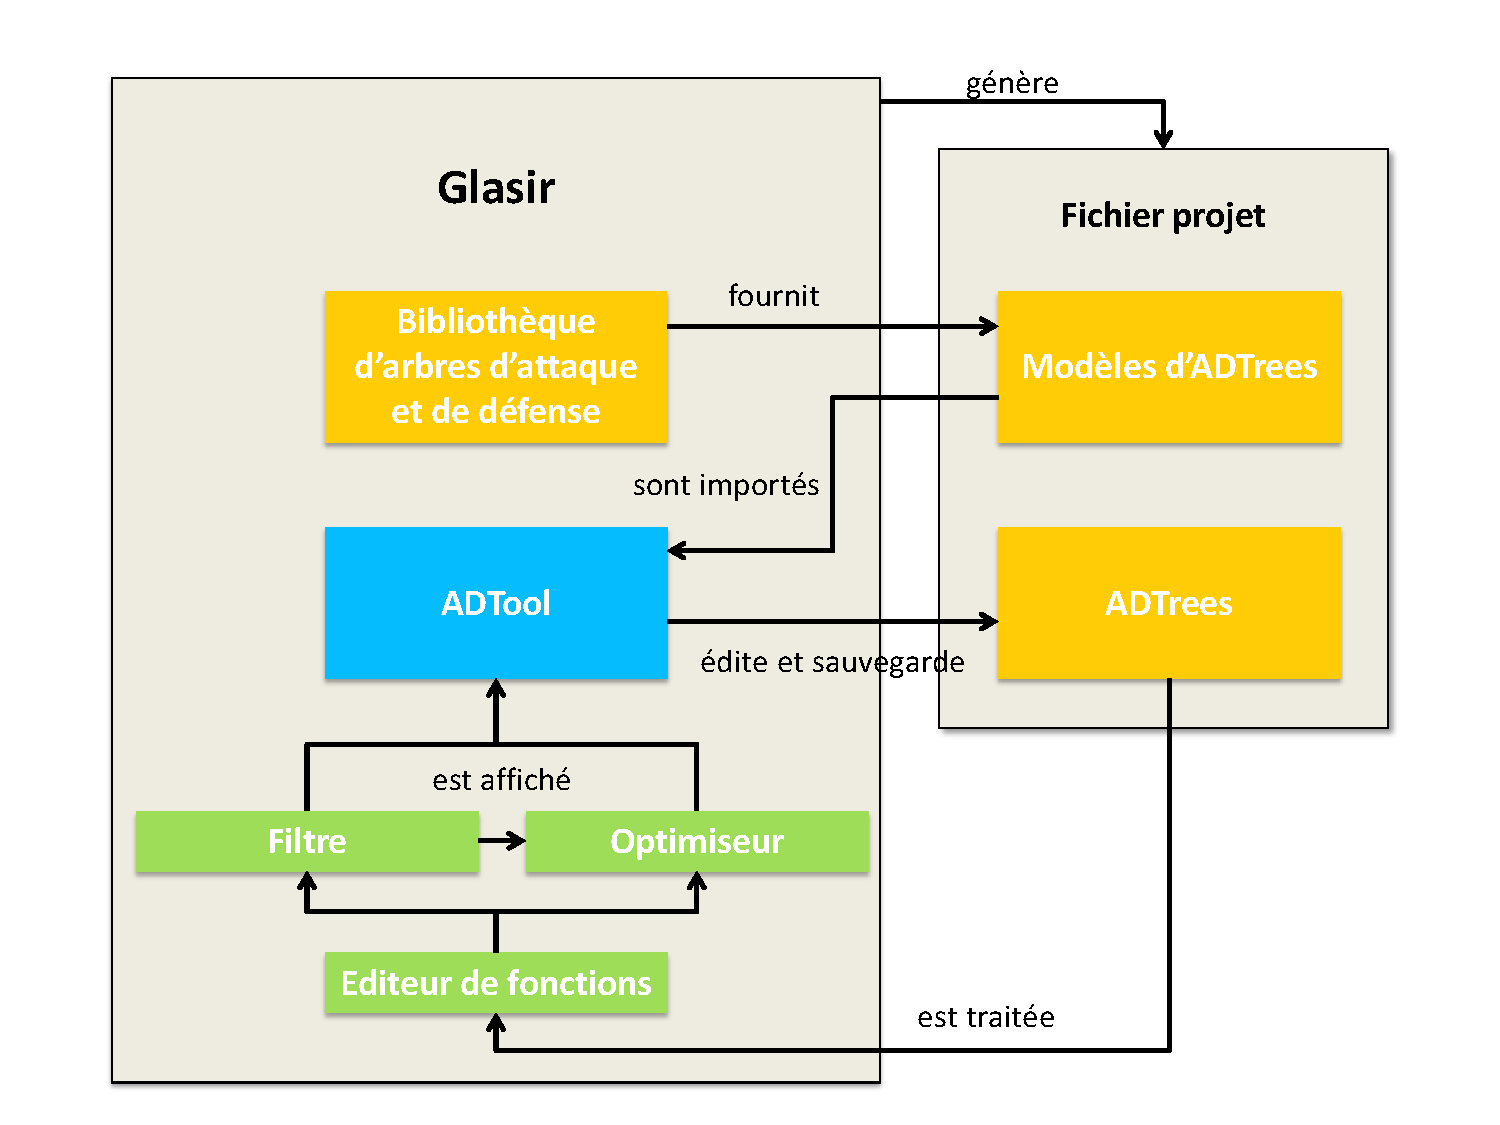
\includegraphics[width=0.8\textwidth]{figure/archiGlasir.pdf}
		\caption{Architecture du logiciel \glasir.}
		\label{fig:architecture_Glasir}
	\end{figure}